%Tapered Stopper
\documentclass[preview]{standalone}
\usepackage{tikz}
\usetikzlibrary{calc}

\begin{document}
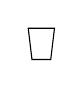
\begin{tikzpicture}
	\pgfmathsetmacro{\R}{1}				%radius of flask
	\pgfmathsetmacro{\neck}{3}			%number of necks
	\pgfmathsetmacro{\pos}{90}			%position of first neck in degrees
	\pgfmathsetmacro{\ang}{45}			%separation of necks in degrees
	\pgfmathsetmacro{\taperwidth}{24}	%Width of the joint taper
	\pgfmathsetmacro{\taperlength}{40}	%Length of the joint taper

	%calculated
	\pgfmathsetmacro{\firstangle}{\pos-\ang}	%Calculating the far right angle
	\pgfmathsetmacro{\secondangle}{\pos+\ang}	%Calculating the far left angle

	\coordinate (a) at ({\pos-atan((\taperwidth/200)/\R)}:\R+\taperlength/100) {};
	\coordinate (b) at ({\pos-atan((\taperwidth/200)/\R)}:\R) [fill=none]{};
	\coordinate (c) at ({\pos+atan((\taperwidth/200)/\R)}:\R) {};
	\coordinate (d) at ({\pos+atan((\taperwidth/200)/\R)}:\R+\taperlength/100) {};

	\draw (a) -- (b) -- (c) -- (d) -- (a) -- (b);

\end{tikzpicture}
\end{document}
